\documentclass[a4paper,12pt]{report}
\addtolength{\oddsidemargin}{-1.cm}
\addtolength{\textwidth}{2cm}
\addtolength{\topmargin}{-2cm}
\addtolength{\textheight}{3.5cm}
\newcommand{\HRule}{\rule{\linewidth}{0.5mm}}
\makeindex

\usepackage{longtable}
\usepackage[pdftex]{graphicx}
\usepackage{makeidx}
\usepackage{hyperref}
\hypersetup{
    colorlinks=true,
    linkcolor=blue,
    filecolor=magenta,      
    urlcolor=cyan,
}


% define the title
\author{Not Like This}
\title{ Network Visualizations interface for large scale networks Functional Requirements}
\begin{document}
\setlength{\parskip}{6pt}

% generates the title
\begin{titlepage}

\begin{center}
% Upper part of the page       
\textsc{\LARGE Department of Computer Science}\\[1.5cm]
\textsc{\Large COS 301 - Software Engineering}\\[0.5cm]
% Title
\HRule \\[0.4cm]

{ \huge \bfseries Not Like This}
\\[0.4cm] 
{ \huge \bfseries Functional Requirements}\\[0.4cm]
\HRule \\[0.4cm]
% Author and supervisor
\begin{minipage}{0.4\textwidth}
\begin{flushleft} \large
\emph{Authors:}
\end{flushleft}
\end{minipage}
\begin{minipage}{0.4\textwidth}
\begin{flushright} \large
\emph{Student number:}
\end{flushright}
\end{minipage}

\begin{minipage}{0.4\textwidth}
\begin{flushleft} \large
Jedd {Shneier}
\end{flushleft}
\end{minipage}
\begin{minipage}{0.4\textwidth}
\begin{flushright} \large
\emph{}
13133064
\end{flushright}
\end{minipage}

\begin{minipage}{0.4\textwidth}
\begin{flushleft} \large
Duncan {Smallwood}
\end{flushleft}
\end{minipage}
\begin{minipage}{0.4\textwidth}
\begin{flushright} \large
\emph{}
13027205
\end{flushright}
\end{minipage}

\begin{minipage}{0.4\textwidth}
\begin{flushleft} \large
Daniel {King}
\end{flushleft}
\end{minipage}
\begin{minipage}{0.4\textwidth}
\begin{flushright} \large
\emph{}
13307607
\end{flushright}
\end{minipage}

\begin{minipage}{0.4\textwidth}
\begin{flushleft} \large
Muller {Potgieter}
\end{flushleft}
\end{minipage}
\begin{minipage}{0.4\textwidth}
\begin{flushright} \large
\emph{}
12003672
\end{flushright}
\end{minipage}


\vfill
% Bottom of the page
{\large \today}
\end{center}
\end{titlepage}
\footnotesize
%\input{declaration_of_originality.tex}
\normalsize

\renewcommand{\thesection}{\arabic{section}}
\newpage
\begin{center}
\textsc{\LARGE Software Requirements Specification and Technology Neutral Process Design}\\[1.5cm]
\textsc{\Large Network Visualizations interface for large scale networks/Main Project}\\[0.5cm]
Version: Version 1.0 Beta
For further references see \href{ https://github.com/u13133064/NotLikeThis}{gitHub}.
\today
\end{center}
\tableofcontents{}
\newpage

\section{Introduction}
This is the Software Requirements specitcation document for a network visuilization system for Amazon web services. Amazon web service customers have hundreds of inter-connected networks with tens-of thousands of networked resources of many types and uses. The Network Visualizations interface for large scale networks (NVI, for short) will be used to create a display of a customer's networks, so that they can have a better understanding of their network. In short a vizualization system to capture the virtual connectiosn between a customers instances within their Amazon Virtual Private Cloud.
The purpose of this document is to capture the functioal and architectural requirments of the system as well as other issues. The document is divided into the following sections:
\begin{enumerate}
	 \setcounter{enumi}{1}
    \item Vision for the system
\begin{itemize}
    \item This includes the projected vision and outcomes of the system and what AWS aims to achieve with this project. 
\end{itemize}

    \item Background to why the system is being developed

\begin{itemize}
    \item This includes a discussion of the problem which AWS has decided upon to address with this project. How this system is intended to solve the problem and why this system is needed.
\end{itemize}
 
    \item Architecture Requirements
\setlength{\parindent}{2.5em}

\begin{itemize}
    \item This includes the software architecture requirements wich include the access and integration requirements, quality
requirements and architectural constraints for the NVI. Additionally to the quality requirements of the system the external systems wich will be incorparated into the system will be discussed. Lastly it will include any constraints that the client has
specifed with regard to technologies used in and by the system.
\end{itemize}


    \item Functional Requirements
\setlength{\parindent}{2.5em}

\begin{itemize}
    \item This section will be expanded opon iteratively in the context of agile software development.
\end{itemize}


    \item Software Requirements
\setlength{\parindent}{2.5em}

\begin{itemize}
    \item This section includes the actual software architecture of the system as well as The strategies, patterns and technologies to be used.This  also includes a discussion on reference technologies and intergration channels.
\end{itemize}



    \item Open Issues
\begin{itemize}
    \item This section will discuss any requirements of the system that may be unclear or has not been specified. It will also include any inconsistencies that have been discovered in the requirements. 
\end{itemize}
\end{enumerate}

\section{Vision}

With the implementation of this system, the client is hoping to reduce the abstraction of the hierarchy of  Amazon Virtual Private network instances and conenctions. The system is to function as a high level rendering of the underlying virtual network architecture. A vizulaization tool to encapsulate the the underlying AWS complexity.

AWS customers have hundreds of inter-connected networks with tens-of thousands of networked resources of many types and uses. Understanding the interplay of all of these pieces on a theoretical level is very difficult and tedious in an actual production environment.

The primary goal of this project is to design and implement novel and interesting patterns and techniques to improve clients understanding of their own networks and understanding of how these networks can be improved and maintained.

Additionally, the system will be used to provide users (who are clients of AWS VPN) with an expandable set of information, of their network, the nodes of the network and indication of how to further improve their network usage and scalability.

A typical usage scenario of the system will be as follows: 

\begin{itemize}
    \item A client logs onto the vizualizer through their AWS account.
\end{itemize}
\begin{itemize}
    \item The vizualizer sends a message to the network scanner containing clients credidentials.
\end{itemize}
\begin{itemize}
    \item The scanner begans traversing the network and updating the vizualizers rendering engine in real time through an asynchronous message communication
\end{itemize}
\begin{itemize}
    \item When the full VPN is scanned or the section the user has a security access too, the scanner decouples from the vizualiser.
\end{itemize}
\begin{itemize}
    \item The user can then interact with the rendered network graph, such as clicking on nodes to expand for more information.
\end{itemize}
\begin{itemize}
    \item The user can also view network speed and resource usage rates.
\end{itemize}




\section{Background}

After tendering for the project our team had a skype meeting with Mr Ivan du Toit at Amazon Web Services situated in Cape Town.
The client discussed with us their wish for a system to To visualise large scale networks and network components including connections and to improve customer understanding by allowing interactive and context sensitive exploration of these networks.
The client emphazized our freedom in coming up with novel solutions to the problem and gave us an explanation of how the system will function within AWS through their EC2 API. We as a team began discussing technologies and the systems architecture as well as study the EC2 documentation and familirize ourselves with the AWS environment. 

We started a  developers blog(http://cos301notlikethis.blogspot.co.za/) to keep each other and the client up to date with ideas and changes. We chose this project beacuse we as a group have an interest in netorks, computer graphics and a desire to work on a large complex system such as AWS. We hope to learn a lot about real world API intergrated development,with a particular desire to learn Amazons' system especially since many of us hoep to work there in the future.

We hope to produce an impressive system that shows off our team members indivual talents, with a goal of improving on the understanding of Amazon clients and making their lives just a bit easier. We also hope to develop a system that meets the high production standards of proffessional companies, and to impress our faculty and peers with our technical skills we been developing these last several years.


\section{Architecture Requirements}
	\subsection{Access Channel Requirements}
		Only registered members of Amazon's EC2 will be allowed to use the visualizer, as it will be integrated into EC2. Clients will be able to use any device(s) that can make use of Chrome, Firefox and/or Internet explorer. The browsers will not need any additional plugins to use the visualizer.
	\subsection{Quality Requirements}
	\begin{enumerate}
		\item The system should show the following performance characteristics:
		\begin{itemize}
			\item Scalability:  It should cater for large and small customers. (The customer's size is in terms of the number of networks[VPCs] and network interfaces)
			\item Performance :The system must work as effciently as possible and not lag in delivering iinformation to the user. The visualization should render all displays in under 10 seconds.
			\item Usability: The project should work within normal EC2 API throttling limits and the site should load and allow customer interaction within 3 seconds on a local network.
			\item  Reliability: It is imperative that the system not experience unnecessary downtime (pe-
riod of in-operation of the system) or problems involving the normal operating parameters of the system. The web page component should require no more computing resources than can be provided without noticeable slow down on a low end consumer laptop.
		\end{itemize}
		\item Security: The system should use secure authentication supported by the EC2 API's and follow best practices 
	\end{enumerate}
	
	\subsection{Integration Requirements}
\begin{enumerate}
    \item GUI
\begin{itemize}
    \item As the system will be accessed remotely through the Internet, it needs to
	integrate with web services. The GUI will be integrated online with HTML,
	JavaScript, CSS and any additional graphic librabries, netowrk libraries and software libraries needed to attain desired functionality. must be intergarted into  Chrome,Firefox and IE web browsers.

\end{itemize}
    \item EC2
\begin{itemize}
    \item Amazon Elastic Compute Cloud (Amazon EC2) is a web service that provides resizable compute capacity in the cloud. It is designed to make web-scale cloud computing easier for developers. The Network scanner needsto be intergrated with the EC2 API and incorporate EC2's security policy. There is a 3 layer intergration with the vizualizer  intergrating with the scanner and the scanner intergrating with the EC2 API.


\end{itemize}

\end{enumerate}
	

All integration needs to be seamless and not interfere with system per-
formance. Security is also a major concern, and thus technologies integrated
must not threaten the system's security as a whole or other technologies.	



	\subsection{Architecture Constraints}
\begin{itemize}
    \item The visualization of the network should be shown in a browser and should only use technology that is supports the latest 3 versions of Chrome, Firefox and Internet explorer

\end{itemize}

\begin{itemize}
    \item The system should require no plugins or add-ons to be installed that is not distributed with the browsers above

\end{itemize}
\begin{itemize}
    \item Users should only be able to see the part of the network they have access too

\end{itemize}
\begin{itemize}
    \item The vizualization must be a hierarchial renddering of the network with expandable information.

\end{itemize}
\begin{itemize}
    \item Must be timely in execution.
\end{itemize}


\section{Functional requirements and Application Design}
This section will be completed ina later stage of development.
	\subsection{Use case prioritization}
	\subsection{Use case/Services contracts}
	\subsection{Required functionality}
	\subsection{Process specifications}
	\subsection{Domain Model}

\section{Software Architecture}
	\subsection{Architectural patterns or styles}
		\subsubsection{Layered Architecture}
		The layered architecture separates various logical layers, specifically in this system the Presentation Layer, The Network Analyser, and The Network. The Network Analyser layer will interact with the Network layer and produce an abstraction of various data with regards to the Network. This is then passed to the Presentation Layer which will create a visual representation of the abstraction produced by the lower level.
		
		Reasons use layered architecture:
		\begin{itemize}
			\item Flexibility, maintainability and scalability. Scalability being a major factor in the overall success of our system. 
			\item It will also allow for teams to work on different parts of the application in parallel, thus speeding up the implentation process. 
			\item It also makes it possible to configure different levels of security to different levels. As some levels require more security than others namely any level dealing with EC2 user's account information.
			\item This also allows for components to be tested independently of each other. 
		\end{itemize}
		
		Some potential issues:
		\begin{itemize}
			\item A major issue with this pattern is that it is possible that it causes a performance decrease as there is an overhead of passing through layers. However, it is still untested and may be nonexistent or negligable.
		\end{itemize}
	\subsection{Architectural tactics or strategies}
		\subsubsection{Performance and Scalability}
		Increased performance and scalability is our main concern as the system needs to be speedy and and not LAG otherwise it is unhelpfull. In order to achieve this we working towards a goal of Managing resource demand through :
		\begin{itemize}
			\item
		Thread Pooling: In thread pooling m threads work on n tasks. Usually m is less than n thus less memory is used for these threads. This will be especially helpful in this system as it will improve scalability which will be needed for the very large networks we will have to work with. 
		
		It can also improve performance as the program no longer has the overhead of creating a new thread for each new task and the system is less likely to have a bottleneck due to high memory usage.
		\end{itemize}
		
\begin{itemize}
			\item
		Caching: Due to the system needing to constantly update caching is going to be extremely useful in increasing the performance of the system, as data can be continiously cached and only updated as time progresses rather than completely replaced with some of the data having not changed at all.
		\end{itemize}
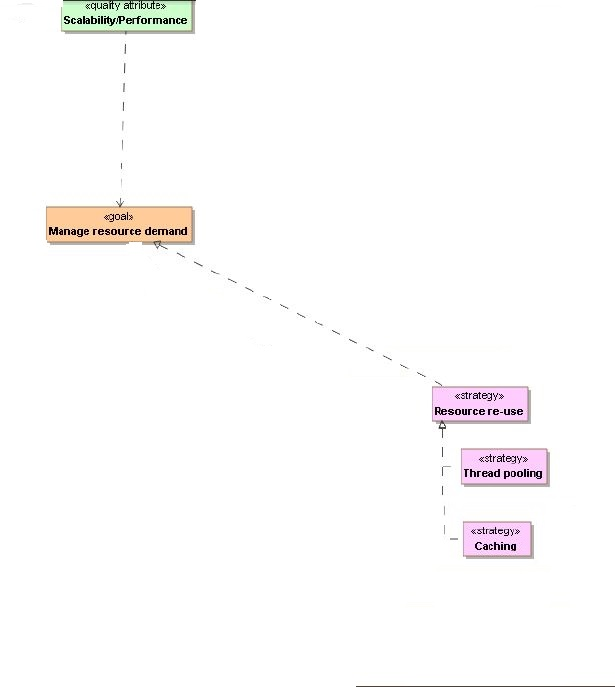
\includegraphics[width=10cm]{./performancefigure.jpg}

		\subsubsection{Reliability}
		In order to maintain reliability we have a goal of preventing faults. In order to prevent faults in the
system, tactics such as error checking and process monitoring are applied.		

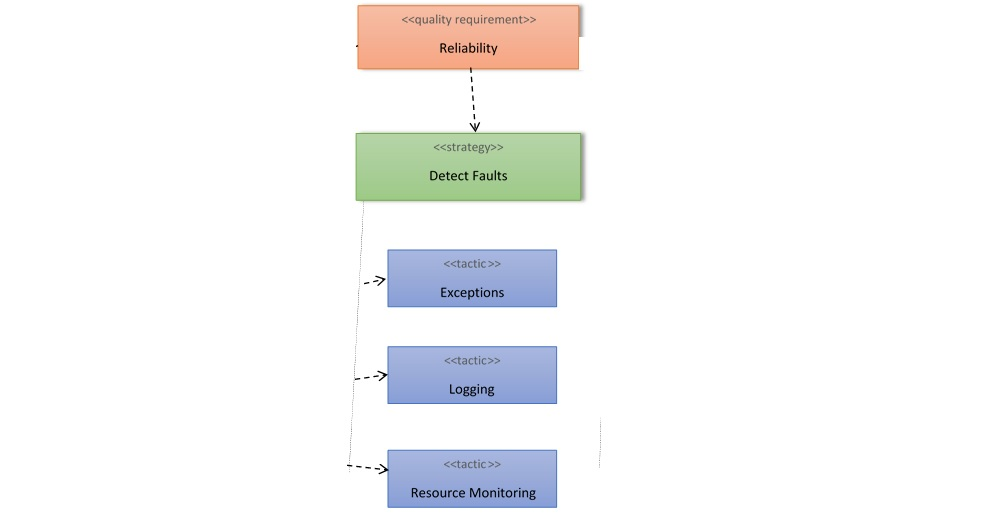
\includegraphics[width=10cm]{./reliabilityfigure.jpg}


		\subsubsection{Security}
		To achieve system security our goal is to resist attacks by limmiting access through strategies of Authorization to deny accessto network sections that user has no access too, Confidentiality to keep sensitive information hidden,Mininimize acccess channels to reduce possible entry vectors of attack and continiuos authentication to maintain identity.

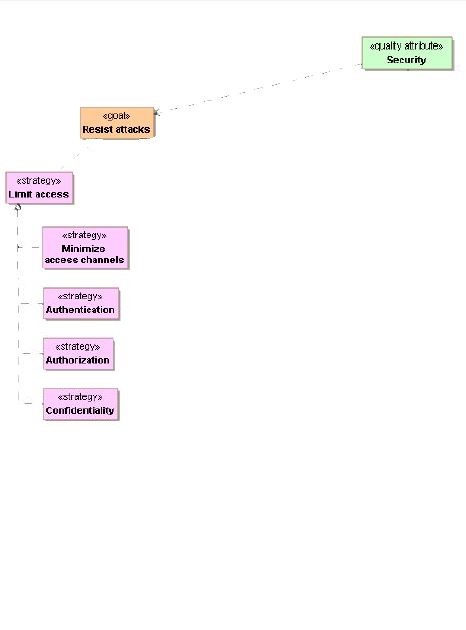
\includegraphics[width=10cm]{./securityfigure.jpg}
	
	
		
	\subsection{Use of reference architectures and frameworks}
	\subsection{Access and integration channels}
		\begin{itemize}
			\item The service will be accessable by human users through any normal web browser.
			\item The service will use Amazon's EC2 API in order to access the information required to perform the service, thus it needs to be able to intergrate with it.
			\item The channels used by EC2 to get its information are already established and their inner workings are beyond the scope of this project, thus they will be ignored.
		\end{itemize}
	\subsection{Technologies}
- HTML: The inter-
face should be represented with HTML5, as it multiplatform and
scalable with future technologies.
- CSS and Bootstrap: Styling the web based interface should be
handled through CSS3 and the Bootstrap framework. Bootstrap
allows for a responsive, mobile interface with a professional ap-
pearance. Importantly its current popularity allows for future
upgrades and scalable interface design.
-Javascript, AngularJS, Three.js and Node.js : The interface needs to remain
robust, intuitive and responsive. To achieve a responsive environ-
ment, AngularJS will be used. Node.js is designed to build scalable
network applications and using these frameworks, our system will
remain modularised and will allow us to implement dependency
injection. For the graphic rendering we will be making use of WebGL through the three.js librarya wich is a cross-browser JavaScript library/API used to create and display animated 3D computer graphics in a web browser using WebGL. 

\section{Open issues}
	\begin{itemize}
		\item The client has yet to mention specific details on how they intend to expand on the base project.
	\end{itemize}
	\begin{itemize}
		\item How many clients should be able to use this system at thye same time?
	\end{itemize}
	\begin{itemize}
		\item Should current rendering be savable. 
	\end{itemize}
	\begin{itemize}
		\item The aesthetics of the vizualizer.
	\end{itemize}
	\begin{itemize}
		\item Should a user be notified when non-authorized user tries to vizualsie their network.
	\end{itemize}
	\begin{itemize}
		\item How much infromation needs to be dispalyed?
	\end{itemize}






\end{document}